\chapter{Continous Integration}
\section{Einleitung}\label{sec:einleitung}
Während des Verlaufes der Diplomarbeit wurde es notwendig unsere Applikation auf einen Server der HTL Leonding zu deployen. Genauer gesagt musste das JavaEE Backen auf einen Application Sever deployed werden. Um jedoch nicht immer per Hand bei der kleinste Änderung das Projekt zu compilieren und dann manuel zu deployen. Wurde entschieden diesen Prozess mithilfe von Continous Integration zu vereinfachen.

\section{Was ist CI?}\label{sec:cierklärung}
Continuous Integration (CI) ist ein Teil der modernen Software Entwicklung. CI stellt den Prozess dar, der das Bauen und Testen einer Anwendung abbildet. Mit Hilfe von CI lassen sich Fehler schneller finden und beheben. Die Idee der kontinuierlichen Integration ist es, dass die Entwickler frühzeitig und regelmäßig Änderungen in das Versionsmanagement einchecken. Diese Änderungen sollten funktionsfähig sein, sodass die gesamte Applikation auf Integrationsprobleme geprüft werden kann.

Es ist somit die Verfügbarkeit einer lauffähigen Version gegeben, die dann z. B. für anderweitige Testzwecke oder Vertriebszwecke genutzt werden kann. Eine typische Anwendung sind sogenannte Nightly Builds, bei denen zu einer vorgegebenen Uhrzeit der aktuelle Programmcode übersetzt wird und dabei Tests mit der erstellten Software automatisch ausgeführt werden. Bei gefundenen Problemen kann ein Entwickler dann z. B. direkt per Mail über das gefundene Problem informiert werden.

\section{Wieso CI?}\label{sec:whyci}
Continuous Integration hat das Ziel, die Qualität der Software über permanente Integration ihrer einzelnen Bestandteile zu steigern. Statt die Software nur in sehr großen Zeitabständen kurz vor der Auslieferung zu erstellen, wird sie in kleinen Zyklen immer wieder erstellt und getestet. Es ist auch ein Zeitgewinn vorhanden da nicht nach jedem Zyklus die Software per Hand sondern auf Knopfdruck ausgeliefert und getestet wird.

\section{Wie kann CI realisiert werden?}\label{sec:whyci}
Folgende Tools kamen für diese Herausforderung in Frage:

\textbf{Bambo}
Bamboo ist ein continuous integration server von Atlassian, den Entwicklern von JIRA, Confluence and Crowd. 

\textbf{Travis CI}

Travis CI ist ein open-source gehosteter, continuous integration Service sehr stark integriert mit Github.

\textbf{Jenkins}

Jenkins ist ein webbasiertes Open Source Continous Integration System. Es ist in Java geschrieben und plattformunabhängig. Die Basis von Jenkins unterstützt zahlreiche Werkzeuge darunter SVN, Ant, Maven sowie JUnit. Durch die Community können weitere Funktionen mit Hilfe von Plugins hinzugefügt werden. Somit lässt sich Jenkins für jedes Projekt individuell anpassen. Auch für Projekte mit anderen Sprachen/Technologien wie z. B. PHP, Ruby oder .NET ist Jenkins geeignet. Testwerkzeuge lassen sich über Plugins über die intuitive Benutzeroberfläche integrieren. Builds können durch verschiedene Auslöser gestartet werden: z. B. Änderung des CVS oder Zeitplan (z. B. Nightly Builds). Nightly Builds sind besonders bei Open Source Projekten zu finden und bedeutet, dass die Applikation nachts gebaut und getestet wird.

Aufgrund der hohen Anpassungsmöglichkeit, großen Community und sehr genauer Dokumentation wurde Jenkins als Tool für die Continous Integration ausgewählt.

\section{Jenkins installieren}
\label{sec:jenkinsinstallation}
Auf unsere Ubuntu 16.04 Server wurde Jenkins mittels Console installiert und zwar musste das Jenkins Apt-Repository dem Server apt-repository hinzugefügt werden mit folgendem Befehl: "wget -q -O - https://pkg.jenkins.io/debian/jenkins-ci.org.key | sudo apt-key add -" und 
"sudo sh -c 'echo deb http://pkg.jenkins.io/debian-stable binary/ > /etc/apt/sources.list.d/jenkins.list'"

Bevor Jenkins installiert wird das Ubuntu Apt-Repository aktualisieren mit "sudo apt-get update" und dann kann jenkins installiert werden mit "sudo apt-get install jenkins".

Nachdem der Installer fertig ist wird wie in der Abbildung\ref{img:consoleoutput} ein initialAdminPassword angezeigt. Dieser wird benötigt um die weiteren Schritte von der Jenkins Installation zu autorisieren.

\begin{figure}[h]
\centering
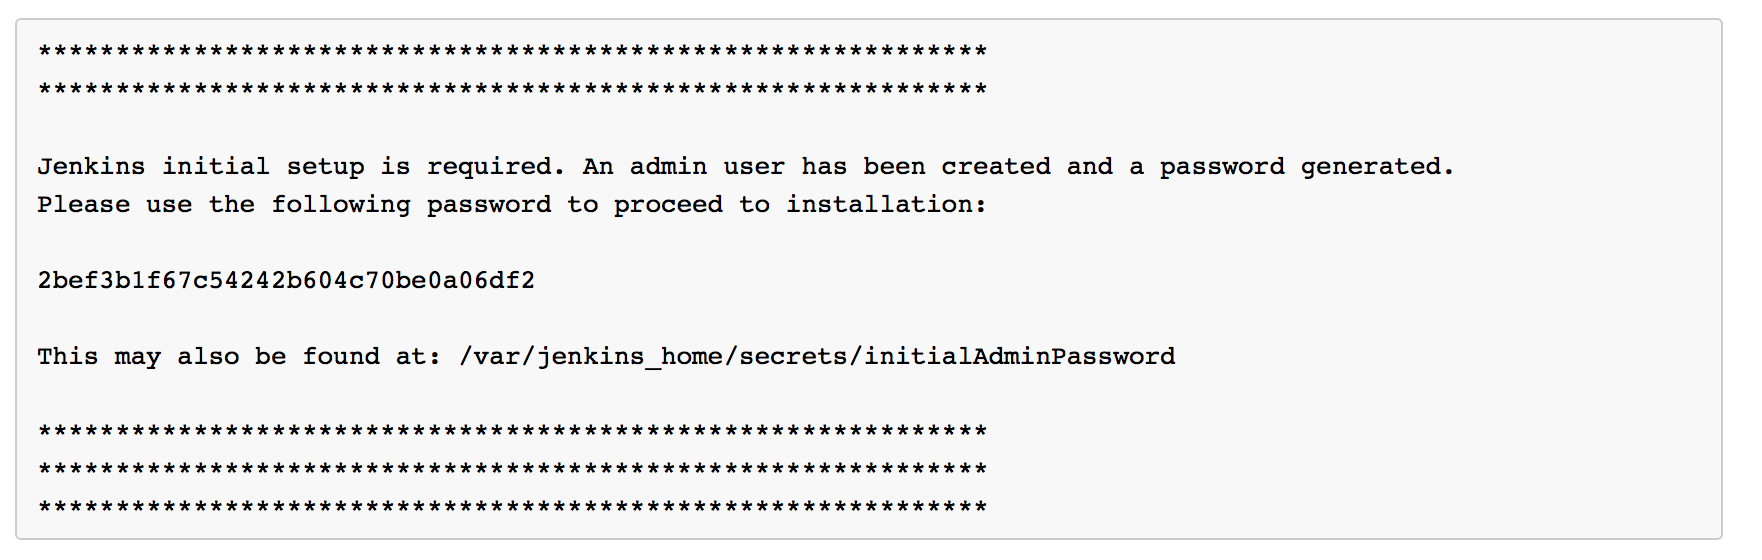
\includegraphics[width=1\textwidth]{images/09_CI/consoleOutput.png}
\caption{Konsolen Ausgabe - Jenkins}
\label{img:consoleoutput}
\end{figure}

Nachdem das initialAdminPassword ausgegeben wurde kann Jenkins unter der ServerUrl  und dem Standard Port 8080 erreicht werden. 

\begin{figure}[h]
\centering
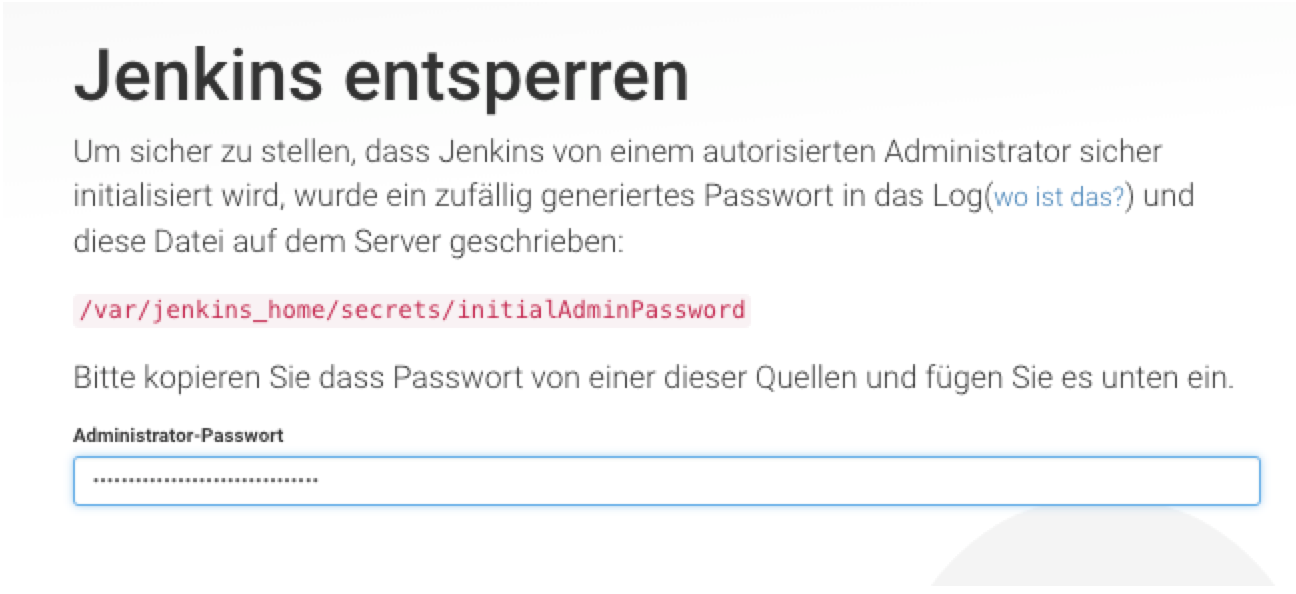
\includegraphics[width=1\textwidth]{images/09_CI/initial.png}
\caption{Anmelden - Jenkins}
\label{img:login}
\end{figure}

Wie in \ref{img:login} muss das Passwort jetzt eingegeben werden um die Installation fortzusetzen. In den nächsten Ansichten muss ein Admin User angelegt werden und die benötigten Plug-Ins für den Jenkins ausgewählt werden. Hier reichen die Standard Plug-Ins völlig aus.

Jetzt kann Jenkins verwendet werden.